\chapter{Planificación y metodología}
\label{planificacion}

\section{Metodología utilizada}
\label{metodologia}
Aunque la realización de este proyecto no requiera en gran medida desarrollar un producto software complejo, 
se ha seguido la metodología de ''Issue Driven Development'' (IDD) con el fin de agilizar y organizar el trabajo.
Se trata de una metodología similar al ''Feature Driven Development'' en la cual la idea principal es que el 
estado actual y futuro del proyecto siempre quede reflejado en el sistema de tracking de issues que esté siendo utilizado.
Esta metodología presenta una serie de ventajas realmente interesantes como la modularidad que proporciona el que 
los commits y las ramas del repositorio sean autocontenidas, la granularidad gracias a que los commits y las ramas 
se centran exclusivamente en una issue actual a cerrar, además de poder llevar registro de las discusiones entre 
colaboradores con respecto a los commits realizados sobre una issue. Aunque esto último no nos atañe debido a que 
el proyecto está siendo desarrollado de forma individual, se trata de un punto positivo muy a tener en cuenta en 
entornos de desarrollo colaborativo.
El "Issue Driven Development" también se caracteriza por seguir una filosofía DRY o ''Don't Repeat Yourself'' en 
la que se incentiva el mantener de forma estructurada, unificada y centralizada toda la información de documentación 
con respecto a cambios y planificación de desarrollo con el fin de evitar problemas de redundancia y posible
fragmentación.

El procedimiento a seguir en esta metodología empieza por la elección de un sistema de gestión de issues. Esto se 
comentará más adelante en ''\nameref{seguimiento}''. A continuación, antes de proceder con la realización de 
cualquier tarea, se crea una issue correspondiente en la quede reflejado qué se desea hacer y cómo se tiene planteado 
hacerlo. Es buena práctica agrupar issues por milestones para tener una visión más general de estas. Una vez 
creadas la issue en cuestión y su milestone correspondiente, se creará una rama en la que se llevará a cabo todo el 
desarrollo relacionado con la issue. Los commits que se realicen a las ramas deberán de contener una descripción 
explicativa de los cambios e incluir en el título una categoría y una referencia a la issue que se está tratando de solucionar. Con 
esto se busca que los commits tengan enlazada toda la información necesaria para comprender fácilmente los cambios 
realizados, es decir, que sean autocontenidos. Por último, una vez que la issue haya sido cerrada a través de un 
commit, se realizará un merge de la rama temática con la rama master.

Como es posible imaginar, esta metodología puede llegar a ser un tanto abrumadora en proyectos pequeños o poco 
complejos en los cuales puede darse el caso de que el esfuerzo de documentar en el sistema de gestión de issues 
todas las tareas a realizar puede llevar más tiempo que la realización de las tareas en sí.

Por último, comentar que para la toma de apuntes sobre la información de interés encontrada y y el desarrollo de 
las pruebas de concepto, se ha utilizado la herramienta de Joplin, una herramienta Open Source multiplataforma que 
permite tomar notas de manera organizada en formato Markdown. El poder mantener un formato constante para los apuntes
realizados en Joplin y los readme del repositorio de trabajo ha sido de gran ayuda para facilitar su traslado.

\section{Temporización}
Para el desarrollo de este proyecto no se ha aplicado una planificación estricta. Desde un principio se estimó una 
duración de tres semanas en base al nivel de conocimiento previo en la materia para la investigación sobre fuzzing,
el estado del arte y diversos posibles casos prácticos
de aplicación del conocimiento obtenido que pudieran ser de interés. Una vez finalizadas, se daría paso a unas cuatro 
semanas para familiarizarnos con las tecnologías y herramientas investigadas además del desarrollo de las pruebas de 
concepto que habían sido fijadas como objetivo. Por último, se estimó una duración de cuatro semanas para la redacción 
y formalización del documento del proyecto y los readme del repositorio.

\section{Seguimiento del desarrollo}
\label{seguimiento}
Github ha sido la plataforma de control de cambios elegida debido a que junto con Git, han sido ampliamente utilizados
en las distintas asignaturas del grado de Ingeniería Informática y ya se parte conociendo su funcionamiento y dinámica de 
trabajo. Github proporciona una funcionalidad de tablero Kanban que combinado con lo comentado en ''\nameref{metodologia}''
nos permite de un vistazo ver el estado actual de las tareas del proyecto mediante su clasificación en una serie de columnas 
definidas que agrupan las issues según si se tratan de issues por comenzar, issues en progreso, issues bloqueadas a espera 
de arreglos en software de terceros o issues completadas.
\begin{figure}
    \vspace*{-2.8in}
    \centering{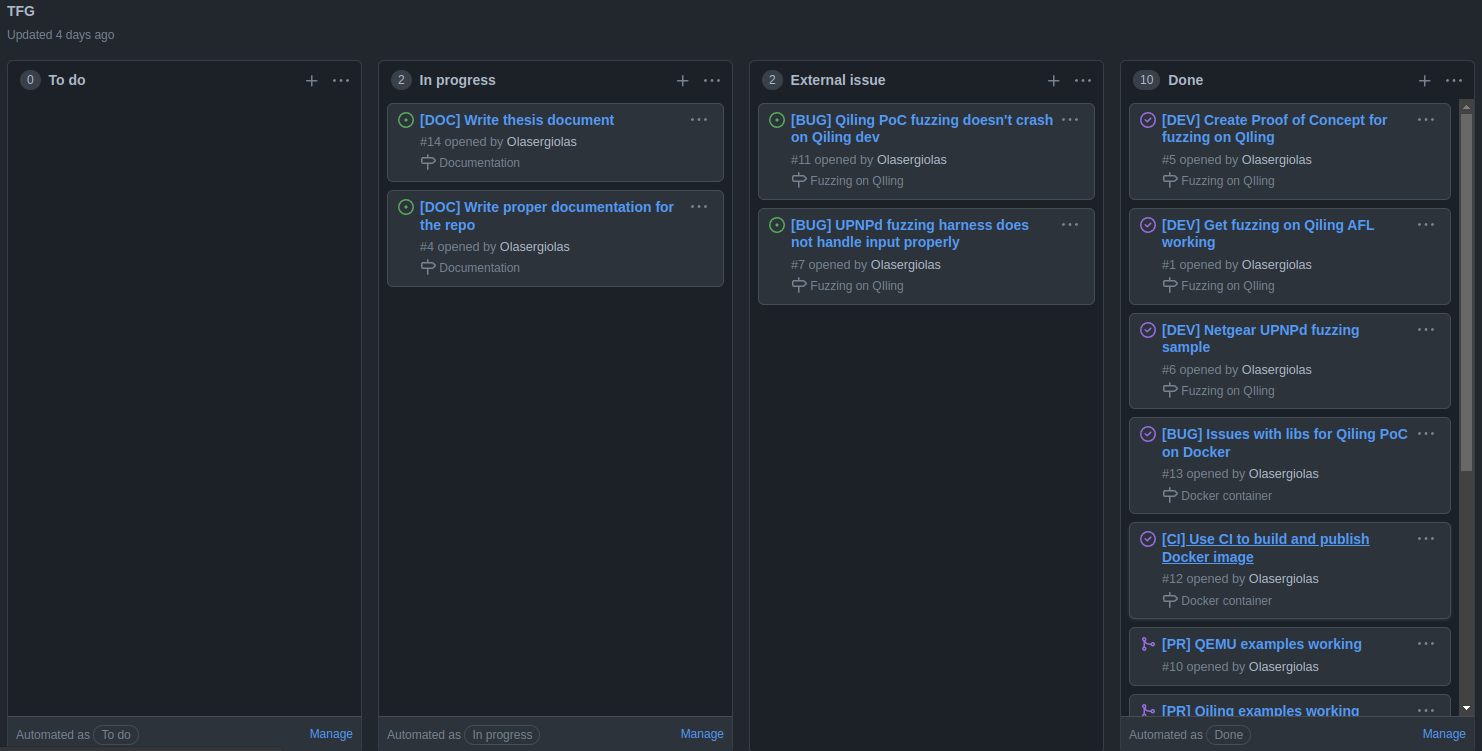
\includegraphics[scale=0.24]{kanban.png}}
    \caption{Funcionalidad de tablero Kanban de Github.}
\end{figure}

\begin{figure}
    \vspace*{-2.8in}
    \centering{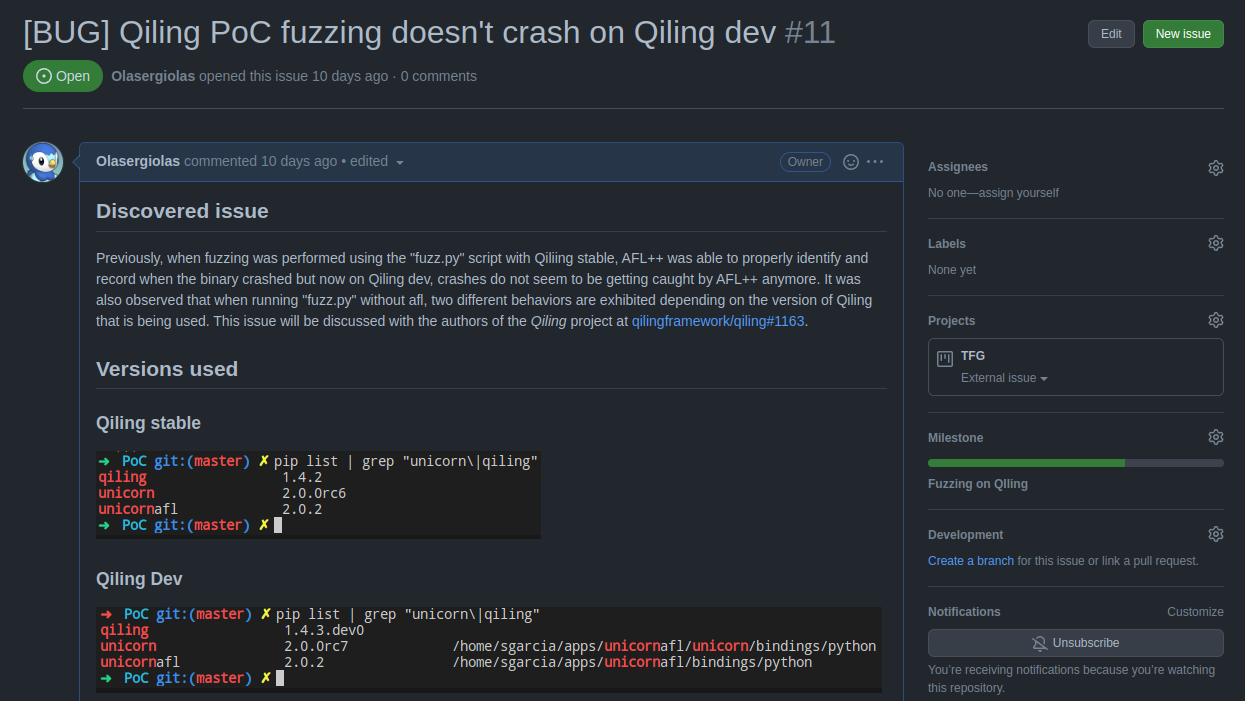
\includegraphics[scale=0.3]{issue.png}}
    \caption{Ejemplo de \href{https://github.com/Olasergiolas/TFG/issues/11}{issue} de reporte de bug en el repositorio del proyecto.}
\end{figure}